\chapter{Thiết kế hệ thống}
\label{Chapter4}

\section{Kiến trúc tổng thể hệ thống}

% TODO: Nội dung (phần này còn để trống trong file Báo Cáo Cuối Kỳ).

\subsection{Mô hình kiến trúc hệ thống}

% TODO: Nội dung.

\subsection{Khái quát các thành phần bên trong hệ thống}

% TODO: Nội dung.

\section{Thiết kế nền tảng Web}

Nền tảng Web của hệ thống được tách thành hai ứng dụng độc lập: ứng dụng web cho người dùng cuối (webapp -- nơi người thuê tìm kiếm, so sánh, lưu tin và liên hệ chủ trọ; đồng thời là không gian để người môi giới/chủ nhà đăng và quản lý tin) và trang quản trị (admin -- dành cho quản trị viên). Mỗi ứng dụng có cơ sở mã, phong cách thiết kế và quy ước kỹ thuật riêng, phù hợp với nhóm người dùng mà nó phục vụ. Phần này tập trung mô tả ứng dụng web cho người dùng cuối, vốn là thành phần người dùng tương tác trực tiếp nhiều nhất; phần trang quản trị được trình bày ở mục tiếp theo.

Webapp được xây dựng trên Next.js 15 (theo mô hình Pages Router) cùng React 19 và TypeScript, sử dụng Tailwind CSS v4 kết hợp bộ component shadcn/ui làm hệ thống giao diện. Việc lựa chọn Next.js cho phép kết xuất phía máy chủ (Server-Side Rendering -- SSR) đối với các trang quan trọng về SEO như trang chi tiết tin đăng và trang tin tức, đồng thời tận dụng được hệ sinh thái React phong phú cho phần tương tác phía trình duyệt \cite{ReactDocs,NextDocs}.

\subsection{Tổ chức mã nguồn}

Mã nguồn được tổ chức theo nguyên tắc \textit{tách bạch mối quan tâm} (separation of concerns) và \textit{thiết kế nguyên tử} (Atomic Design), với mục tiêu để mỗi tính năng có thể phát triển độc lập, dễ kiểm thử và dễ bảo trì. Toàn bộ mã nguồn nằm dưới thư mục \texttt{src/}, được phân chia thành các nhóm chính như Bảng~\ref{tab:webapp-structure}.

\begin{table}[H]
\centering
\caption{Cấu trúc thư mục mã nguồn của ứng dụng web}
\label{tab:webapp-structure}
\begin{tabular}{|L{0.30\textwidth}|L{0.60\textwidth}|}
\hline
\textbf{Thư mục} & \textbf{Vai trò} \\
\hline
\texttt{pages/} & Lớp định tuyến (Pages Router). Mỗi tệp là một ``vỏ mỏng'' chỉ lắp ghép dữ liệu vào template và gắn bố cục trang. \\
\hline
\texttt{components/} & Cây giao diện theo Atomic Design: \texttt{atoms} (nguyên tử shadcn), \texttt{molecules}, \texttt{organisms}, \texttt{templates} và \texttt{layouts}. \\
\hline
\texttt{api/services/} & Các module gọi API theo từng nghiệp vụ (tin đăng, môi giới, thanh toán, tin tức, thông báo, AI\ldots). \\
\hline
\texttt{hooks/} & Các React Hook tùy biến đóng gói logic nghiệp vụ và truy vấn dữ liệu. \\
\hline
\texttt{contexts/}, \texttt{store/} & Quản lý trạng thái dùng chung (xác thực, ngôn ngữ, danh sách so sánh\ldots) qua React Context và Zustand. \\
\hline
\texttt{configs/}, \texttt{constants/} & Cấu hình thư viện (axios, biến môi trường) và hằng số toàn cục. \\
\hline
\texttt{messages/}, \texttt{utils/}, \texttt{styles/} & Bộ từ điển đa ngôn ngữ, các hàm tiện ích thuần và mã định kiểu giao diện. \\
\hline
\end{tabular}
\end{table}

Cây giao diện tuân thủ nghiêm ngặt thứ tự phân lớp \texttt{atoms $\to$ molecules $\to$ organisms $\to$ templates $\to$ pages}, trong đó lớp dưới không bao giờ được phép nhập (import) từ lớp trên. Cụ thể, \texttt{atoms} là các nguyên tử giao diện cơ bản (nút bấm, ô nhập liệu, hộp thoại\ldots) được chuẩn hóa theo shadcn/ui; \texttt{molecules} ghép các nguyên tử thành các khối nhỏ như trường biểu mẫu, thẻ lọc; \texttt{organisms} là các khối tính năng hiểu biết về dữ liệu và quy tắc nghiệp vụ (thẻ tin đăng, hộp thoại đăng nhập, widget trợ lý AI\ldots); \texttt{templates} là bố cục đầy đủ của một họ trang; còn \texttt{pages} chỉ đóng vai trò lắp ráp. Mỗi thư mục thành phần đều cung cấp một tệp \texttt{index} làm điểm xuất khẩu tập trung (barrel export), giúp việc nhập khẩu nhất quán và che giấu cấu trúc nội bộ.

Song song với cây giao diện, logic được tách theo \textit{nghiệp vụ}: mỗi miền dữ liệu có một module dịch vụ (\texttt{*.service.ts}) chịu trách nhiệm gọi API và một nhóm hook (\texttt{use*}) bao bọc dịch vụ đó. Nhờ vậy, logic nghiệp vụ nằm ở hook và context, việc lấy dữ liệu nằm ở tầng dịch vụ, còn component chỉ lo phần hiển thị. Cách phân tách này giúp giảm thiểu sự phụ thuộc chéo và cho phép nhiều thành viên cùng phát triển các tính năng khác nhau mà ít xảy ra xung đột.

Hình~\ref{fig:webapp-source-org} tổng hợp cách tổ chức mã nguồn webapp theo các lớp nêu trên. Lớp định tuyến (\texttt{pages}) nằm trên cùng; bên dưới là cây giao diện Atomic Design (\texttt{templates $\to$ organisms $\to$ molecules $\to$ atoms}) tách biệt với nhánh logic gồm \texttt{hooks}, \texttt{contexts}/\texttt{store} và tầng dịch vụ (\texttt{api/services}) chịu trách nhiệm gọi API qua \texttt{axios}. Mũi tên nét liền thể hiện quan hệ phụ thuộc khi kết xuất giao diện, còn mũi tên nét đứt thể hiện việc các thành phần sử dụng hook để lấy dữ liệu; nhờ đó component chỉ lo phần hiển thị, còn logic nghiệp vụ và truy xuất dữ liệu được đẩy xuống các tầng phía dưới.

\begin{figure}[H]
\centering
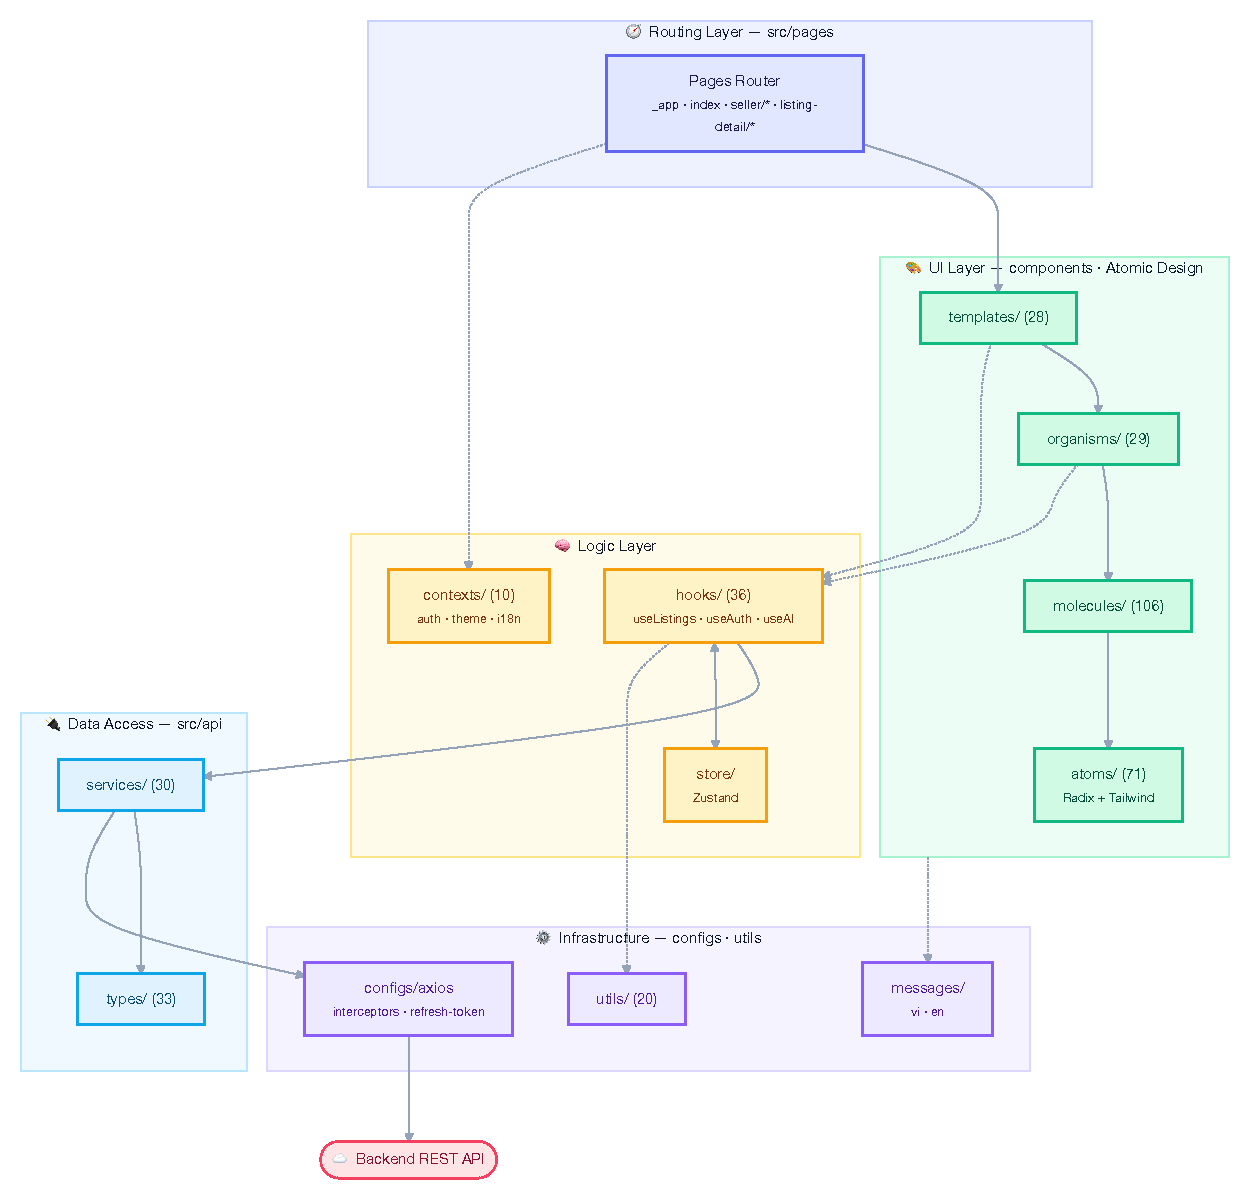
\includegraphics[width=\textwidth]{../diagrams/fe/pdf/01-architecture-layers}
\caption{Sơ đồ tổ chức mã nguồn ứng dụng web (webapp)}
\label{fig:webapp-source-org}
\end{figure}

\subsection{Cơ chế kết nối và tích hợp}

Ứng dụng web không tự chứa dữ liệu mà kết nối tới nhiều dịch vụ phía sau thông qua các kênh giao tiếp được chuẩn hóa:

\begin{itemize}
\item \textbf{Giao tiếp HTTP với Backend chính.} Mọi yêu cầu REST đi qua một thể hiện \texttt{axios} duy nhất được cấu hình tập trung tại \texttt{src/configs/axios}. Thể hiện này gắn sẵn URL gốc của Backend (biến môi trường \texttt{URL\_API\_BASE}), tiêu đề mặc định và bộ chặn (interceptor) xử lý xác thực. Toàn bộ phản hồi được chuẩn hóa về một kiểu \texttt{ApiResponse} thống nhất để các tầng phía trên xử lý nhất quán.

\item \textbf{Xác thực bằng JWT và cơ chế làm mới token.} Bộ chặn yêu cầu tự động đính kèm access token vào tiêu đề \texttt{Authorization}. Khi token sắp hết hạn hoặc máy chủ trả về lỗi 401, hệ thống tự động gọi refresh token để lấy token mới rồi phát lại yêu cầu ban đầu một cách trong suốt với người dùng. Cơ chế này còn khử trùng lặp (deduplication) để nhiều yêu cầu đồng thời chỉ kích hoạt đúng một lần làm mới, tránh tình trạng đua tranh (race condition).

\item \textbf{Cổng chặn truy cập (middleware).} Tệp \texttt{src/middleware.ts} đóng vai trò cổng kiểm soát: nó cho phép một danh sách các tuyến công khai (trang chủ, danh sách tin, chi tiết tin, tin tức, bản đồ\ldots) và chặn các tuyến cá nhân khi người dùng chưa đăng nhập. Khi đó, người dùng được chuyển hướng kèm tham số \texttt{returnUrl} để sau khi đăng nhập có thể quay lại đúng trang đang truy cập.

\item \textbf{Bộ nhớ đệm dữ liệu máy chủ.} Toàn bộ trạng thái lấy từ máy chủ được quản lý bởi TanStack Query, giúp tự động lưu đệm, làm mới nền và đồng bộ dữ liệu giữa các thành phần. Một số dữ liệu thống kê ổn định theo ngày (ví dụ thống kê tin theo tỉnh thành) còn được lưu bền vào \texttt{localStorage} để tồn tại qua các lần tải lại trang.

\item \textbf{Kết nối dịch vụ AI bằng luồng SSE.} Trợ lý hội thoại AI kết nối tới một dịch vụ AI riêng (biến môi trường \texttt{URL\_API\_AI}) và nhận câu trả lời theo thời gian thực qua kỹ thuật Server-Sent Events -- SSE (sử dụng thư viện \texttt{fetch-event-source}). Nhờ đó nội dung trả lời hiện dần theo từng đoạn, kèm theo trạng thái công cụ mà AI đang thực thi, và người dùng có thể hủy luồng đang chạy.

\item \textbf{Thông báo thời gian thực qua WebSocket.} Các thông báo (tin được duyệt, có người quan tâm\ldots) được đẩy theo thời gian thực qua giao thức STOMP trên SockJS, kết hợp với cơ chế hỏi vòng (polling) dự phòng khi mất kết nối.

\item \textbf{Tích hợp dịch vụ bên thứ ba.} Bản đồ tin đăng tích hợp Google Maps; luồng thanh toán điều hướng sang cổng thanh toán rồi nhận lại kết quả qua một trang callback công khai để cổng có thể chuyển hướng về.
\end{itemize}

Hình~\ref{fig:webapp-data-flow} minh họa luồng dữ liệu điển hình khi thực hiện một thao tác đọc/ghi: thành phần giao diện gọi hook, hook ủy thác cho TanStack Query, qua tầng dịch vụ và \texttt{axios} (kèm bộ chặn tự đính kèm và làm mới token) trước khi tới Backend. Khi ghi dữ liệu thành công, hook chủ động vô hiệu hóa bộ đệm liên quan (\texttt{invalidateQueries}) để dữ liệu hiển thị được làm mới một cách nhất quán.

\begin{figure}[H]
\centering
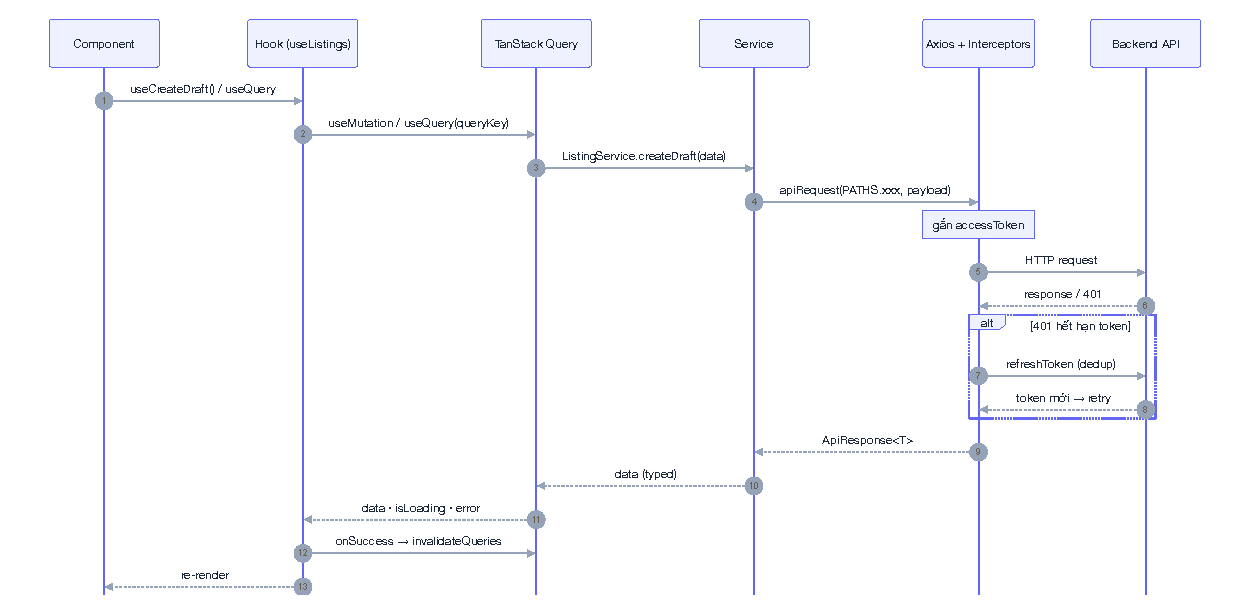
\includegraphics[width=0.92\textwidth]{../diagrams/fe/pdf/04-data-flow}
\caption{Luồng dữ liệu giữa giao diện, hook, tầng dịch vụ và Backend}
\label{fig:webapp-data-flow}
\end{figure}

\subsection{Hỗ trợ đa ngôn ngữ}

Ứng dụng hỗ trợ song ngữ tiếng Việt (mặc định) và tiếng Anh, được triển khai bằng thư viện next-intl. Mọi chuỗi hiển thị cho người dùng -- nhãn, nút bấm, thông báo, thông điệp lỗi, văn bản trạng thái rỗng -- đều không được viết cứng trong mã mà phải lấy qua các hàm \texttt{useTranslations} (phía client) hoặc \texttt{getTranslations} (phía server), tham chiếu tới hai bộ từ điển \texttt{messages/vi.json} và \texttt{messages/en.json}.

Một số điểm kỹ thuật đáng chú ý trong cơ chế đa ngôn ngữ:

\begin{itemize}
\item \textbf{Tải từ điển theo nhu cầu.} Vì phần lớn người dùng sử dụng tiếng Việt, bộ từ điển \texttt{vi.json} được đóng gói sẵn cùng ứng dụng; bộ \texttt{en.json} chỉ được tải động khi người dùng thực sự chuyển sang tiếng Anh, giúp giảm kích thước gói tải ban đầu.
\item \textbf{Bảo đảm đồng bộ khóa dịch.} Một kịch bản kiểm tra (\texttt{check-i18n-keys.js}) được chạy tự động trong bước \texttt{pre-commit} để đối chiếu sự tương đồng khóa giữa hai tệp ngôn ngữ; nếu thiếu khóa ở một ngôn ngữ, thao tác commit sẽ bị chặn.
\item \textbf{Dùng định dạng ICU.} Các chuỗi có tham số sử dụng placeholder kiểu ICU (\texttt{\{name\}}, \texttt{\{count, plural, \ldots\}}) thay vì nối chuỗi thủ công, bảo đảm đúng ngữ pháp khi trật tự từ khác nhau giữa các ngôn ngữ.
\item \textbf{Quản lý trạng thái ngôn ngữ.} Việc chuyển ngôn ngữ được điều phối qua một context riêng (\texttt{SwitchLanguageProvider}), ghi nhớ lựa chọn của người dùng và cung cấp bộ từ điển phù hợp cho toàn bộ cây thành phần.
\end{itemize}

Hình~\ref{fig:webapp-i18n} minh họa cùng một trang chủ được hiển thị ở hai ngôn ngữ: tiếng Việt (mặc định) và tiếng Anh. Người dùng có thể chuyển đổi tức thời thông qua bộ chọn ngôn ngữ trên thanh điều hướng mà không cần tải lại trang; toàn bộ nhãn, nút bấm và nội dung tĩnh đều được thay thế theo bộ từ điển tương ứng.

\begin{figure}[H]
\centering
\includegraphics[width=0.88\textwidth]{giao-dien-ngon-ngu-viet}\\[4pt]
{\small (a) Giao diện tiếng Việt}\\[10pt]
\includegraphics[width=0.88\textwidth]{giao-dien-ngon-ngu-anh}\\[4pt]
{\small (b) Giao diện tiếng Anh}
\caption{Giao diện trang chủ hiển thị ở hai ngôn ngữ tiếng Việt và tiếng Anh}
\label{fig:webapp-i18n}
\end{figure}

\subsection{Ưu điểm}

Cách tổ chức và tích hợp nêu trên mang lại một số ưu điểm rõ rệt cho nền tảng web:

\begin{itemize}
\item \textbf{Dễ bảo trì và mở rộng.} Kiến trúc Atomic Design phân lớp rõ ràng cùng việc tách logic theo nghiệp vụ giúp định vị và sửa đổi mã nhanh chóng; thêm một tính năng mới thường chỉ cần bổ sung một template, một dịch vụ và một nhóm hook tương ứng mà không ảnh hưởng phần còn lại.
\item \textbf{An toàn kiểu dữ liệu.} Việc dùng TypeScript trên toàn dự án, giới hạn kiểu \texttt{any} chỉ trong tầng định nghĩa dữ liệu truyền tải, giúp phát hiện sớm lỗi ngay khi biên dịch.
\item \textbf{Hiệu năng và trải nghiệm tốt.} Kết hợp SSR cho các trang trọng yếu về SEO, tải động (lazy loading) các thành phần nặng như bản đồ và biểu đồ, cùng cơ chế lưu đệm của TanStack Query giúp trang hiển thị nhanh và mượt.
\item \textbf{Nhất quán về giao diện.} Hệ thống thiết kế tập trung (typography, khoảng cách, màu sắc theo token ngữ nghĩa) cùng các quy tắc lint riêng bảo đảm giao diện đồng nhất giữa các trang và giữa các thành viên phát triển.
\item \textbf{Thuận lợi cho cộng tác nhóm.} Quy ước thư mục, barrel export và các cổng kiểm soát chất lượng (lint, kiểm tra kiểu, kiểm tra khóa đa ngôn ngữ) tạo nền tảng để nhiều người cùng làm việc trên cùng mã nguồn mà vẫn giữ được chất lượng ổn định.
\end{itemize}

\section{Thiết kế hệ thống Backend}

% Ghi chú: phần §3.3 do Ty + Tường phụ trách. Các sơ đồ và đoạn giải thích dưới đây
% được soạn sẵn (nháp) kèm hình minh họa; Ty + Tường rà soát, chỉnh và bổ sung nội dung.

Backend của hệ thống được xây dựng trên Spring Boot 3.4 (Java) và đóng gói thành một khối triển khai duy nhất theo mô hình Modular Monolith: toàn bộ nghiệp vụ chạy trong cùng một tiến trình nhưng được chia thành nhiều module theo miền nghiệp vụ, với ranh giới được giữ rõ ràng ở mức gói (package) và tầng dịch vụ. Cách tiếp cận này vẫn giữ được sự đơn giản khi vận hành và gỡ lỗi của một monolith, đồng thời đạt mức tách bạch đủ tốt để nhiều thành viên cùng phát triển song song.

\subsection{Kiến trúc Modular Monolith}

Hình~\ref{fig:be-architecture} mô tả kiến trúc phân lớp của Backend. Mọi yêu cầu từ web, di động hay trang quản trị đi vào qua tầng API gồm 54 controller (\texttt{@RestController}, đa số định tuyến theo tiền tố \texttt{/v1}); sau khi qua bộ lọc bảo mật, yêu cầu được chuyển xuống tầng dịch vụ (chứa toàn bộ logic nghiệp vụ), rồi tới tầng truy xuất dữ liệu (\texttt{repository}) và cơ sở dữ liệu MySQL. Bao quanh các tầng là những mối quan tâm xuyên suốt (cross-cutting): xác thực OAuth2 kết hợp JWT, bộ đệm Redis và cơ chế chịu lỗi Resilience4j.

\begin{figure}[H]
\centering
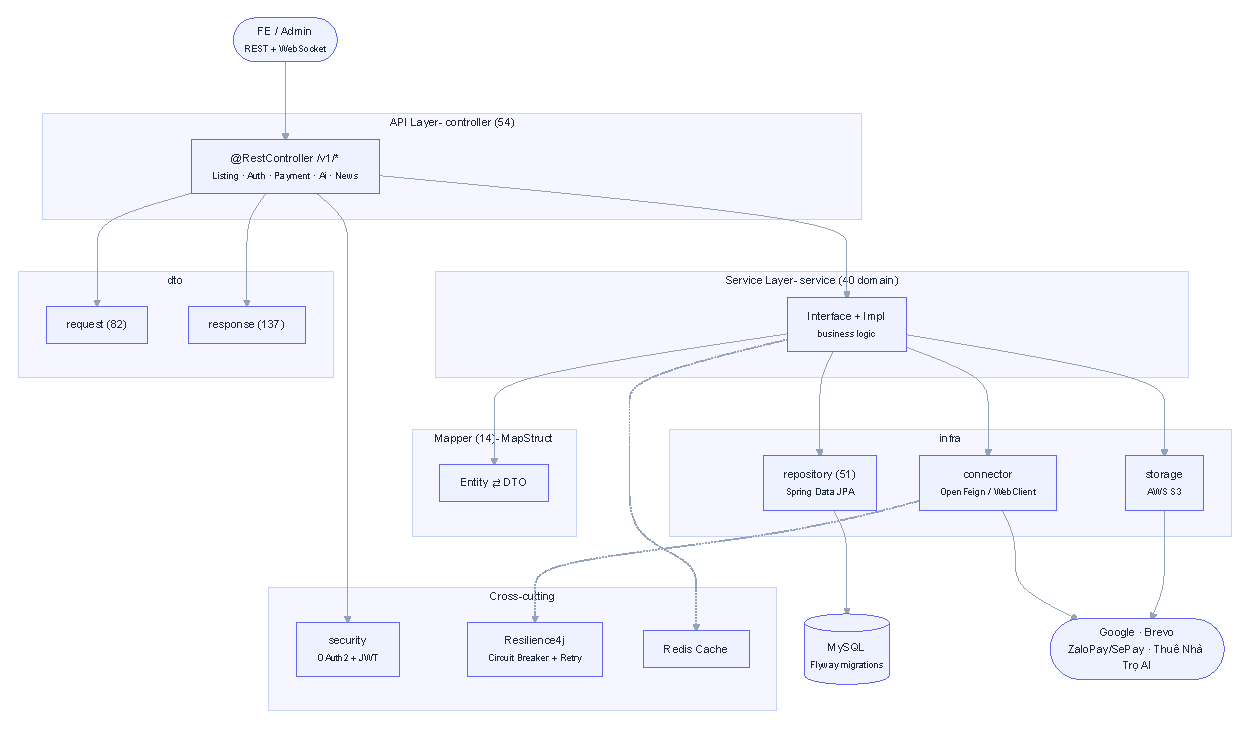
\includegraphics[width=\textwidth]{../diagrams/be/pdf/01-architecture-layers}
\caption{Kiến trúc phân lớp của hệ thống Backend (Modular Monolith)}
\label{fig:be-architecture}
\end{figure}

Tuy là một monolith nhưng hệ thống không cô lập: nó kết nối tới nhiều dịch vụ bên ngoài thông qua tầng \texttt{connector} (OpenFeign/WebClient) và \texttt{storage}, như tóm tắt ở Hình~\ref{fig:be-integrations} -- gồm MySQL, Redis, lưu trữ đối tượng (S3), đăng nhập và định vị qua Google, gửi email (Brevo), cổng thanh toán (ZaloPay/SePay) và dịch vụ AI riêng.

\begin{figure}[H]
\centering
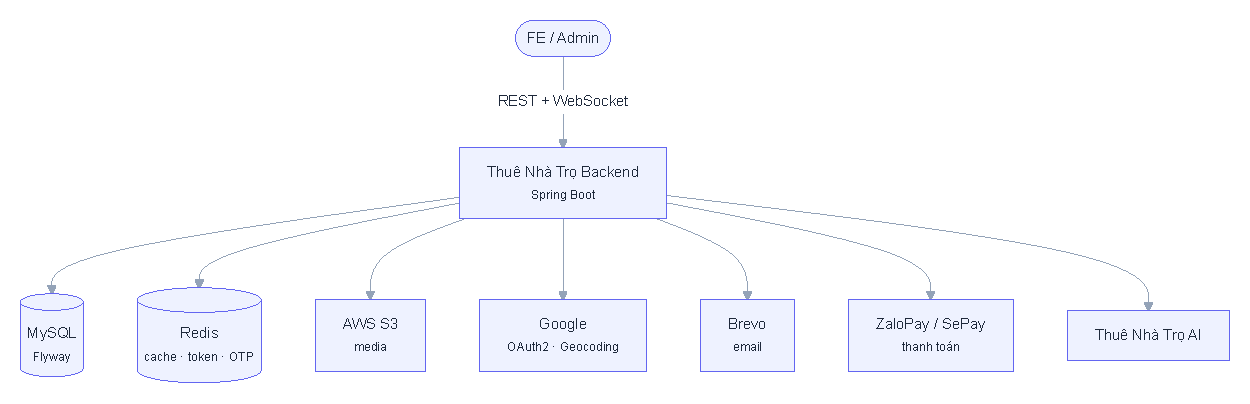
\includegraphics[width=0.95\textwidth]{../diagrams/be/pdf/05-external-integrations}
\caption{Các dịch vụ bên ngoài mà Backend tích hợp}
\label{fig:be-integrations}
\end{figure}

\subsection{Các module nghiệp vụ}

Phần nghiệp vụ được chia thành khoảng 40 module dịch vụ, mỗi module phụ trách một miền độc lập. Hình~\ref{fig:be-domains} nhóm các module theo năm cụm chức năng chính: (i) nghiệp vụ cốt lõi về tin đăng, danh mục, tìm kiếm và định giá; (ii) người dùng và xác thực; (iii) thanh toán và gói thành viên; (iv) tương tác và nội dung (thông báo, email, tin tức, AI); và (v) vận hành (quản trị, kiểm duyệt, thống kê hành vi).

\begin{figure}[H]
\centering
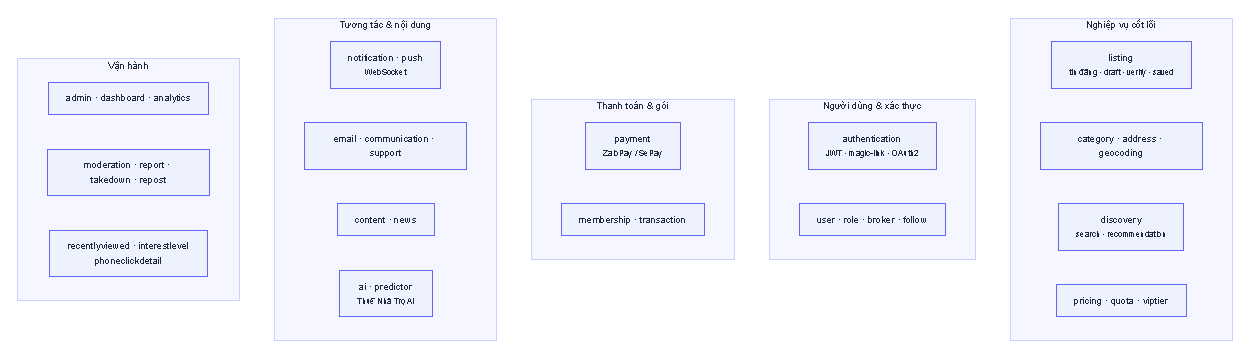
\includegraphics[width=\textwidth]{../diagrams/be/pdf/04-domain-modules}
\caption{Các module nghiệp vụ của Backend gom theo cụm chức năng}
\label{fig:be-domains}
\end{figure}

\subsection{Tổ chức phân tầng bên trong module}

Bên trong mỗi module, mã nguồn tuân theo cùng một khuôn phân tầng nhất quán, phản ánh qua cấu trúc gói \texttt{com.smartrent} ở Hình~\ref{fig:be-packages}. Tầng \texttt{controller} chỉ tiếp nhận yêu cầu và kiểm tra hợp lệ dữ liệu (\texttt{@Valid}); tầng \texttt{service} (tách giao diện và phần hiện thực \texttt{impl}) chứa logic nghiệp vụ; \texttt{mapper} (MapStruct) chuyển đổi giữa thực thể và DTO; còn \texttt{infra/repository} dùng Spring Data JPA để truy xuất dữ liệu. Các đối tượng truyền tải được tách thành \texttt{dto/request} và \texttt{dto/response}, trong khi cấu hình hệ thống (bảo mật, cache, circuit breaker, WebSocket) nằm trong gói \texttt{config}. Bảng~\ref{tab:backend-structure} liệt kê chi tiết vai trò của từng gói chính trong mã nguồn Backend.

\begin{table}[H]
\centering
\caption{Cấu trúc gói mã nguồn của Backend (\texttt{com.smartrent})}
\label{tab:backend-structure}
\begin{tabular}{|L{0.26\textwidth}|L{0.64\textwidth}|}
\hline
\textbf{Gói} & \textbf{Vai trò} \\
\hline
\texttt{controller/} & Lớp API: 54 lớp \texttt{@RestController} expose các REST endpoint (đa số theo tiền tố \texttt{/v1}); tiếp nhận yêu cầu, kiểm tra hợp lệ dữ liệu và ủy thác cho tầng dịch vụ. \\
\hline
\texttt{service/} & Lớp nghiệp vụ: 40 module theo miền (tin đăng, xác thực, thanh toán, AI\ldots), mỗi module tách \textit{giao diện} và phần \textit{hiện thực} (\texttt{impl}). \\
\hline
\texttt{dto/} & Đối tượng truyền tải, tách \texttt{request} (82) và \texttt{response} (137); cách ly mô hình API khỏi thực thể cơ sở dữ liệu. \\
\hline
\texttt{mapper/} & 14 bộ chuyển đổi (MapStruct) giữa thực thể (entity) và DTO. \\
\hline
\texttt{infra/} & Hạ tầng truy xuất dữ liệu và tích hợp: \texttt{repository} (51 -- Spring Data JPA), \texttt{connector} (gọi dịch vụ ngoài qua OpenFeign/WebClient), \texttt{storage} (S3), \texttt{client}. \\
\hline
\texttt{config/} & Cấu hình hệ thống: \texttt{security} (OAuth2 + JWT), \texttt{cache} (Redis), \texttt{circuitbreaker} (Resilience4j), WebSocket, S3 và cổng thanh toán. \\
\hline
\texttt{enums/}, \texttt{constants/} & 31 kiểu liệt kê và các hằng số nghiệp vụ dùng chung. \\
\hline
\texttt{exception/} & Các ngoại lệ nghiệp vụ và bộ xử lý lỗi tập trung (\texttt{GlobalPaymentExceptionHandler}). \\
\hline
\texttt{cronjob/} & Tác vụ định kỳ: tự kiểm duyệt tin bằng AI, thông báo tin sắp hết hạn, làm mới bộ đệm thống kê trang chủ. \\
\hline
\texttt{util/}, \texttt{utility/}, \texttt{validator/} & Hàm tiện ích (sinh \texttt{Snowflake} ID, chuẩn hóa văn bản tìm kiếm, dựng email, che dữ liệu nhạy cảm) và bộ kiểm tra ràng buộc (số tiền, hạn mức). \\
\hline
\end{tabular}
\end{table}

Cấu trúc gói nói trên được minh họa trực quan ở Hình~\ref{fig:be-packages}.

\begin{figure}[H]
\centering
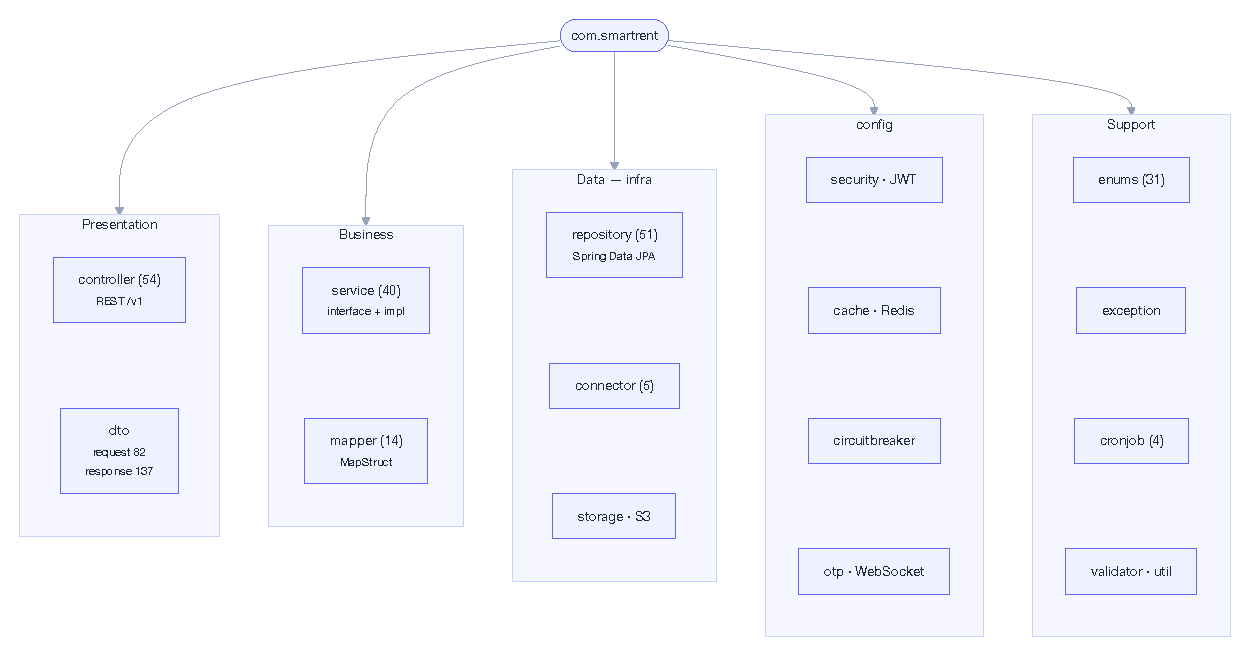
\includegraphics[width=\textwidth]{../diagrams/be/pdf/02-package-structure}
\caption{Cấu trúc gói \texttt{com.smartrent} và cách phân tầng}
\label{fig:be-packages}
\end{figure}

\subsection{Luồng dữ liệu}

Hình~\ref{fig:be-request-flow} minh họa luồng xử lý một yêu cầu có xác thực. Yêu cầu kèm \textit{Bearer token} trước hết đi qua bộ lọc bảo mật để \texttt{CustomJwtDecoder} kiểm tra token; controller kiểm tra hợp lệ DTO rồi gọi service. Service ưu tiên đọc từ bộ đệm Redis, chỉ truy vấn cơ sở dữ liệu khi \textit{cache miss} và ghi lại kết quả vào đệm; sau đó dùng mapper chuyển thực thể sang DTO phản hồi và trả về cho client dưới dạng \texttt{ApiResponse} JSON.

\begin{figure}[H]
\centering
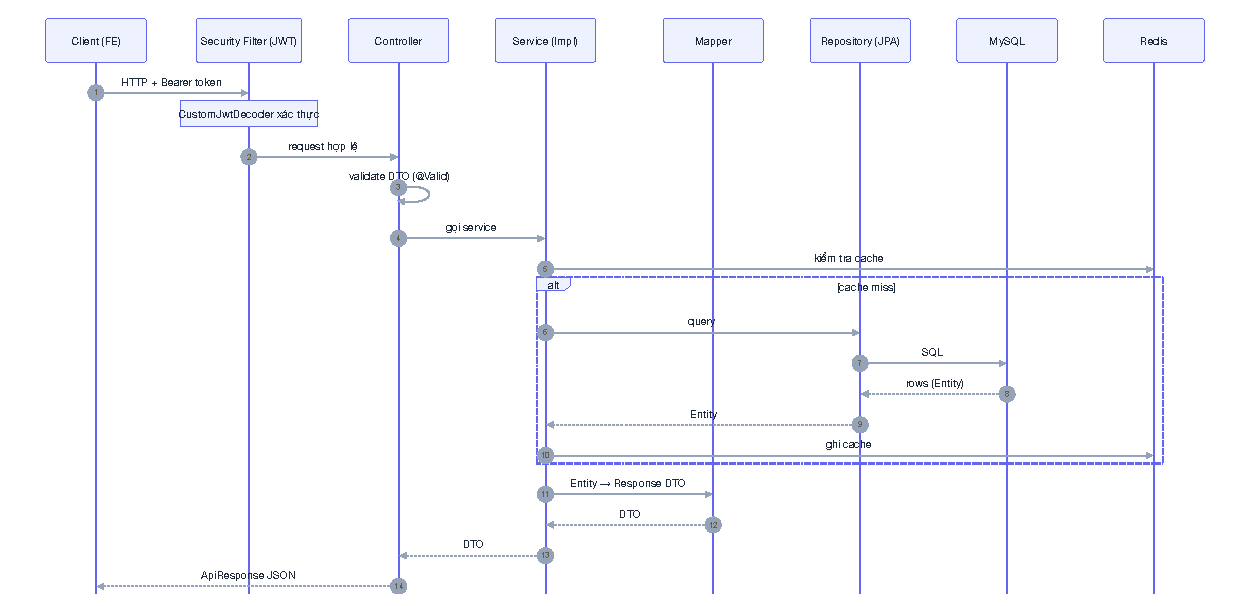
\includegraphics[width=\textwidth]{../diagrams/be/pdf/03-request-flow}
\caption{Luồng xử lý một yêu cầu có xác thực ở Backend}
\label{fig:be-request-flow}
\end{figure}

\subsection{Ưu điểm}

Mô hình Modular Monolith mang lại một số ưu điểm cho Backend của hệ thống:

\begin{itemize}
\item \textbf{Đơn giản khi vận hành.} Một khối triển khai duy nhất giúp việc build, kiểm thử và gỡ lỗi dễ dàng, đồng thời giảm chi phí hạ tầng so với kiến trúc microservices.
\item \textbf{Tách bạch theo miền.} Ranh giới module rõ ràng cho phép nhiều thành viên cùng phát triển song song mà ít giẫm chân lên nhau.
\item \textbf{Nhất quán phân tầng.} Cùng một khuôn \texttt{controller--service--repository} ở mọi module giúp mã dễ đọc, dễ bảo trì và rút ngắn thời gian làm quen cho thành viên mới.
\item \textbf{Chịu lỗi và hiệu năng.} Bộ đệm Redis giảm tải truy vấn cơ sở dữ liệu, còn Resilience4j (circuit breaker và retry) cô lập sự cố từ các dịch vụ bên ngoài, giữ hệ thống ổn định.
\item \textbf{Bảo mật tập trung.} Cơ chế xác thực OAuth2 kết hợp JWT được áp dụng thống nhất ở tầng lọc, tách khỏi logic nghiệp vụ.
\end{itemize}

\section{Thiết kế kiến trúc AI}

% TODO: Nội dung (mục mới bổ sung theo cấu trúc báo cáo).

\subsection{Luồng xử lý AI Chatbot}

% TODO: Nội dung.

\subsection{Luồng gợi ý phòng trọ}

% TODO: Nội dung.

\subsection{Tích hợp API AI}

% TODO: Nội dung.

\subsection{Kiến trúc tích hợp AI}

% TODO: Nội dung.

\section{Thiết kế cơ sở dữ liệu}

% TODO: Nội dung.

\subsection{Giới thiệu tổng quan}

% TODO: Nội dung.

\subsection{Sơ đồ thiết kế cơ sở dữ liệu của hệ thống chính}

% TODO: Nội dung.

\subsection{Mô tả chi tiết các bảng}

% TODO: Nội dung.

\section{Thiết kế giao diện}

% TODO: Nội dung (mục mới bổ sung theo cấu trúc báo cáo).

\subsection{Giao diện người thuê}

Giao diện dành cho người thuê được thiết kế đáp ứng (responsive) trên mọi kích thước màn hình, lấy người tìm trọ làm trung tâm của hành trình trải nghiệm. Toàn bộ giao diện kế thừa một hệ thống thiết kế (design system) thống nhất: bảng màu, kiểu chữ, bo góc và khoảng cách đều được khai báo dưới dạng \textit{token ngữ nghĩa} thông qua các biến CSS (CSS custom properties) trong \texttt{styles/globals.css}, thay vì gán giá trị màu cứng tại từng thành phần. Nhờ đó, hệ thống hỗ trợ sẵn hai chế độ sáng/tối (light/dark) chỉ bằng cách hoán đổi nhóm biến, và giữ được sự đồng nhất về thị giác giữa các trang cũng như giữa các thành viên phát triển.

Về kiểu chữ, ứng dụng dùng bộ phông hỗ trợ tốt cả tiếng Việt lẫn tiếng Anh (Be~Vietnam~Pro làm phông chính, Inter và Plus~Jakarta~Sans cho tiêu đề), tải qua cơ chế tối ưu phông của Next.js để tránh hiện tượng nhấp nháy khi tải. Các thành phần giao diện được xây trên nền shadcn/ui kết hợp Tailwind CSS v4, bảo đảm khả năng truy cập (accessibility) và tính nhất quán của nút bấm, biểu mẫu, hộp thoại, thẻ thông tin\ldots

Bố cục chung của khu vực người thuê được gói trong một \textit{layout} dùng lại cho hầu hết các trang, gồm: thanh điều hướng trên cùng (header) chứa logo, thanh tìm kiếm, bộ chuyển ngôn ngữ, chuông thông báo và khu vực tài khoản; phần nội dung ở giữa; chân trang (footer) với các liên kết phụ trợ; và một thanh nổi so sánh hiển thị khi người dùng đang chọn tin để đối chiếu. Cách bố trí này giúp người dùng luôn truy cập nhanh các chức năng cốt lõi ở bất kỳ trang nào.

Một số nguyên tắc thiết kế giao diện được áp dụng xuyên suốt khu vực người thuê:

\begin{itemize}
\item \textbf{Phản hồi trạng thái rõ ràng.} Mỗi thao tác bất đồng bộ đều có trạng thái tương ứng: khung chờ dạng \textit{skeleton} khi đang tải dữ liệu, chỉ báo tiến trình khi chuyển trang, thông báo lỗi thân thiện và \textit{trạng thái rỗng} có hướng dẫn khi không có kết quả.
\item \textbf{Tải động thành phần nặng.} Các khối tốn tài nguyên như bản đồ, biểu đồ lịch sử giá và danh sách tin tương tự được tải động (lazy loading) kèm khung chờ, giúp nội dung chính hiển thị nhanh mà không bị chặn.
\item \textbf{Bố cục thích ứng.} Trên màn hình lớn, trang danh sách tin dùng bố cục hai cột (bộ lọc cạnh kết quả); trên thiết bị di động, bộ lọc thu gọn vào hộp thoại trượt để tiết kiệm không gian.
\item \textbf{Đa ngôn ngữ.} Mọi nhãn, thông báo và văn bản hiển thị đều đi qua lớp đa ngôn ngữ Việt~--~Anh, cho phép chuyển đổi tức thời mà không cần tải lại trang; việc đổi ngôn ngữ chỉ thay đổi nội dung chữ, không đổi đơn vị tiền tệ của giá.
\end{itemize}

Các màn hình chính của người thuê -- trang chủ, danh sách/tìm kiếm tin, chi tiết tin đăng, bản đồ, so sánh, tin đã lưu, trang theo dõi người đăng và tin tức -- đều tuân theo cùng bộ nguyên tắc trên; kết quả hiện thực cụ thể của từng màn hình được trình bày ở Chương~\ref{Chapter5} (phần kết quả giao diện dành cho người thuê).

\subsection{Giao diện chủ trọ}

% TODO: Nội dung.

\subsection{Giao diện quản trị}

% TODO: Nội dung.

\subsection{Giao diện chatbot AI}

% TODO: Nội dung.
